\documentclass[12pt,a4paper,oneside]{report}
\usepackage[T1]{fontenc}
\usepackage[utf8]{inputenc}
\usepackage{newtxtext,newtxmath}
\usepackage[left=32mm,right=25mm,top=25mm,bottom=25mm,headheight=16pt]{geometry}
\usepackage{setspace,microtype,graphicx,pdfpages,float,placeins}
\usepackage{booktabs,longtable,tabularx,array,multirow}
\usepackage{amsmath,enumitem,xcolor,listings,titlesec,fancyhdr}
\usepackage{tikz}
\usetikzlibrary{arrows.meta,positioning,shapes.geometric,fit,backgrounds,calc}
\usepackage[numbers,sort&compress]{natbib}
\usepackage[hidelinks,bookmarksnumbered,pdfpagelabels]{hyperref}
\usepackage{bookmark}
\usepackage[font=small,labelfont=bf,skip=8pt]{caption}
\renewcommand{\bibname}{References}
\hypersetup{pdftitle={NEXOS AI Assisted Linux Distribution Project Report},pdfauthor={NEXOS Project Team},pdfsubject={Major Project I architecture implementation and evaluation plan}}
\graphicspath{{images/}}
\onehalfspacing
\setlength{\parindent}{1.2em}
\setlength{\parskip}{4pt}
\setlength{\emergencystretch}{2em}
\widowpenalty=10000
\clubpenalty=10000
\raggedbottom
\setcounter{tocdepth}{1}
\setcounter{secnumdepth}{2}
\setlist{itemsep=3pt,topsep=5pt,parsep=0pt}
\renewcommand{\arraystretch}{1.25}
\newcolumntype{Y}{>{\raggedright\arraybackslash}X}
\newcolumntype{P}[1]{>{\raggedright\arraybackslash}p{#1}}
\titleformat{\chapter}[display]{\normalfont\bfseries\Large}{CHAPTER \thechapter}{9pt}{\LARGE}
\titlespacing*{\chapter}{0pt}{-8pt}{22pt}
\titleformat{\section}{\normalfont\large\bfseries}{\thesection}{0.7em}{}
\titleformat{\subsection}{\normalfont\normalsize\bfseries}{\thesubsection}{0.7em}{}
\pagestyle{fancy}
\fancyhf{}
\fancyhead[L]{\small NEXOS}
\fancyhead[R]{\small Major Project I}
\fancyfoot[C]{\thepage}
\renewcommand{\headrulewidth}{0pt}
\fancypagestyle{plain}{\fancyhf{}\fancyfoot[C]{\thepage}\renewcommand{\headrulewidth}{0pt}}
\definecolor{navy}{HTML}{17324D}
\definecolor{pale}{HTML}{EDF2F6}
\definecolor{ink}{HTML}{202A34}
\lstset{basicstyle=\ttfamily\footnotesize,breaklines=true,columns=fullflexible,keepspaces=true,showstringspaces=false,frame=single,rulecolor=\color{black!25},xleftmargin=5pt,xrightmargin=5pt,aboveskip=10pt,belowskip=10pt}
\tikzset{box/.style={draw=navy,rounded corners=2pt,fill=pale,align=center,font=\small,minimum height=11mm,text width=37mm,inner sep=5pt},flow/.style={-{Latex[length=2mm]},thick,draw=navy},labeltext/.style={font=\scriptsize,fill=white,inner sep=2pt}}
\newcommand{\frontchapter}[1]{\chapter*{#1}\phantomsection\addcontentsline{toc}{chapter}{#1}}
\newcommand{\reportfigure}[4]{\begin{figure}[htbp]\centering\includegraphics[width=#2\textwidth]{#1}\caption{#3}\label{#4}\end{figure}}
\begin{document}
\hypersetup{pageanchor=false}
% The first three pages are fixed exports from the supplied DOCX.
% A missing export deliberately stops the final build.
\includepdf[pages=1-3,fitpaper=true,pagecommand={}]{source/first-three-pages.pdf}
\hypersetup{pageanchor=true}
\pagenumbering{roman}
\frontchapter{Declaration}
We declare that this project report, entitled \emph{NEXOS AI Powered Agentic Operating System}, presents our proposed design and the implementation work identified in the report. The ideas, methods and documentation taken from other sources are acknowledged through citations and references. We have distinguished completed work from proposed work and have not represented planned capabilities, illustrative interfaces or evaluation targets as measured results.

We understand that academic integrity requires accurate attribution, reproducible evidence and truthful reporting of project progress. The architectural diagrams and interface concepts prepared for this report communicate the NEXOS design; they do not constitute evidence that all depicted components have been implemented.

\vspace{18mm}
\begin{tabularx}{\textwidth}{Y l}
\textbf{Project group member} & \textbf{Signature}\\[7mm]
Sandesh Brahmane & \rule{45mm}{0.4pt}\\[7mm]
Omkar Sonawane & \rule{45mm}{0.4pt}\\[7mm]
Mahesh Patil & \rule{45mm}{0.4pt}\\[7mm]
Sarvesh Mane & \rule{45mm}{0.4pt}
\end{tabularx}
\vfill
\noindent Date: \rule{35mm}{0.4pt}\hfill Place: \rule{45mm}{0.4pt}
\clearpage
\frontchapter{Acknowledgements}
We thank Smt. Indira Gandhi College of Engineering, Ghansoli, for the academic environment and facilities supporting this major project. We acknowledge our supervisor, Dr. Madhu Nashipudimath, for guidance in defining the project scope, organizing the technical work and developing the report.

We thank the Department of CSE IoT and Cyber Security including Blockchain, its faculty members and the project review panel for their guidance and feedback. Their emphasis on clear objectives, sound engineering practice and evidence based evaluation has helped shape the direction of NEXOS.

We also acknowledge the researchers and open source communities whose work provides the foundations for this project. Ubuntu, the Linux ecosystem, Python, Qt, SQLite, Ollama and the cited agent research enable the investigation of an integrated workstation automation system within the resources of an undergraduate project.

\vspace{15mm}
\begin{flushright}
Sandesh Brahmane\\Omkar Sonawane\\Mahesh Patil\\Sarvesh Mane
\end{flushright}
\clearpage
\frontchapter{Abstract}
NEXOS is a proposed AI assisted Linux distribution for bounded and verifiable workstation automation. The project integrates a native desktop assistant, a local task engine and model inference with an existing Ubuntu 24.04 LTS operating system. Its purpose is to convert selected natural language requests into observable outcomes while keeping execution subject to explicit permissions, typed tool contracts and independent result checks. The project develops application and distribution integration in user space and reuses the upstream Linux kernel, drivers, networking and desktop infrastructure.

The proposed architecture contains a Qt interface, a Python background service, a model gateway, a dependency aware scheduler, specialist agent roles, a permission broker, isolated tool workers and a SQLite state store. A model proposes structured actions; deterministic software validates and authorizes them. Local tools operate on granted resources, while external service actions use dedicated connectors and account authorization. Verification compares the resulting artifacts or service state with task specific postconditions before success is reported.

An initial implementation provides static inspection of selected Python and Node.js manifests, scoped report creation, hash based evidence checks and persistent task records. Ten foundation tests have passed on Windows and Ubuntu WSL, and a foundation Debian package has been built and checked through extraction. Natural language planning, the native desktop, Linux worker isolation and the bootable distribution remain implementation milestones. These early checks do not establish end to end agent accuracy or complete system security.

The planned deliverable is a customized Ubuntu ISO containing the NEXOS software and first run configuration. Evaluation will measure verified task completion, permission enforcement, latency, resource use, recovery and clean installation behavior. The expected contribution is a reproducible integration and evaluation approach for a small set of useful workstation tasks on constrained student hardware.

\noindent\textbf{Keywords:} agentic systems, Linux distribution, large language models, capability control, task orchestration, outcome verification, ISO packaging.
\clearpage
\frontchapter{Abbreviations and Notation}
\begin{longtable}{P{25mm}P{115mm}}
\toprule\textbf{Term} & \textbf{Meaning}\\\midrule\endhead
AI & Artificial intelligence\\API & Application programming interface\\CPU & Central processing unit\\DAG & Directed acyclic graph\\DFD & Data flow diagram\\FTS5 & SQLite full text search extension version 5\\GPU & Graphics processing unit\\IPC & Interprocess communication\\ISO & Bootable optical disc image used as installation media\\JSON & JavaScript Object Notation\\LLM & Large language model\\LTS & Long term support\\OAuth & Authorization framework used by external service connectors\\QML & Declarative interface language used by Qt Quick\\RAM & Random access memory\\SHA256 & Secure Hash Algorithm producing a 256 bit digest\\TCB & Trusted computing base\\UEFI & Unified Extensible Firmware Interface\\VM & Virtual machine\\WSL & Windows Subsystem for Linux\\$G=(V,E)$ & Task graph with steps $V$ and dependency edges $E$\\$C$ & Set of capabilities granted to a task\\$P_i$ & Postconditions required for step $i$\\\bottomrule
\end{longtable}

\tableofcontents
\clearpage
\phantomsection\addcontentsline{toc}{chapter}{List of Figures}\listoffigures
\clearpage
\phantomsection\addcontentsline{toc}{chapter}{List of Tables}\listoftables
\clearpage
\pagenumbering{arabic}
\chapter{Introduction}
\section{Project Context}
Workstation tasks often span several applications and require a sequence of small decisions. A developer may locate a project, inspect its manifest, identify a runtime requirement, examine prepared service information and assemble a report. A student organizing a review meeting may collect attendees, select a time, create an event and confirm that a meeting link exists. Existing operating systems provide the mechanisms for these actions, but users must coordinate them through interfaces, commands and application specific knowledge.

Language models offer a way to express the intended outcome in ordinary language. However, producing a plausible explanation is different from safely changing files or creating an external event. An agent must select the right resources, interpret the request, obey its granted authority, handle failures and determine whether the requested outcome actually occurred. These requirements motivate NEXOS: an integrated Linux environment in which selected automation workflows are visible, bounded and verifiable.

NEXOS is an Ubuntu based distribution with a native assistant and a local execution service. Ubuntu supplies the operating system substrate; NEXOS supplies the automation layer and its integration. The term \emph{agentic operating system} describes the intended user experience and orchestration layer. It does not imply a newly written kernel or a replacement for Linux process scheduling.

\section{Problem Definition}
The central engineering problem is to translate a user request into a sequence of authorized operations and to establish, using evidence, whether those operations achieved the requested state. Natural language may omit a destination, timezone, project identity or overwrite preference. A retrieved document may contain misleading instructions. A model may select an unsupported tool or produce invalid arguments. A tool may time out after partially completing an operation. A polished final answer alone cannot resolve these conditions.

The problem is therefore defined as follows: given an intent, a declared set of resources and a finite execution budget, construct and execute a valid plan through registered adapters, persist its state and verify its postconditions without exceeding granted capabilities. When the goal cannot be completed, the system must return a specific incomplete or failed outcome and preserve enough evidence for investigation.

\section{Motivation and Intended Users}
The initial users are students and developers working on small local projects. These users benefit from a consistent workflow for inspecting project metadata and generating a report. This starting point is intentionally narrow: source manifests can be read without running the project, outputs can be placed in a known directory, and correctness can be checked against explicit fixtures.

The longer term motivation is to make routine workstation actions easier to request and review. A useful assistant should reduce repetitive coordination while leaving the user able to understand the proposed effect. Action previews, progress updates and evidence links are therefore part of the product design, rather than decorative interface additions.

No general claim is made that existing assistants cannot act or that conventional Linux automation lacks verification. Scripts, service managers, configuration tools and modern agents already automate substantial work. NEXOS investigates a particular combination of local deployment, a native interface, constrained adapters and outcome checks in a reproducible student project.

\section{Objectives and Contributions}
The primary objectives are to:
\begin{enumerate}
\item provide a native interface for requesting and inspecting bounded tasks;
\item validate model proposals against a finite tool registry and explicit schemas;
\item enforce per task resource permissions before dispatching work;
\item persist task progress and distinguish execution from verification;
\item integrate the software into installable packages and a bootable Ubuntu ISO;
\item evaluate functional behavior, adverse inputs, recovery and resource use.
\end{enumerate}

The intended contribution is an engineered prototype and its evaluation evidence. It combines known techniques rather than claiming a new foundational model, a novel Linux kernel or a universal security solution. A successful final project will show a complete path from request to checked outcome on a declared set of tasks and will document the limits of that path.

\section{Scope and Report Organization}
The first workflow inspects Python and Node.js project manifests and creates a verified report. Subsequent workflows add selected file operations, named user service inspection and a Google Calendar connector. Voice interaction, broad visual desktop control and larger plugin ecosystems are extension topics. Arbitrary root commands, unattended financial transactions and unrestricted background monitoring are outside the initial scope.

The report first reviews relevant research and defines requirements. It then develops the architecture, execution model, security boundary, data design and user interface. Later chapters describe the implemented foundation, packaging approach, evaluation protocol and development roadmap. Appendices provide concrete interface examples, test fixtures and release criteria. Planned interfaces and algorithms are specifications until an implementation and corresponding test evidence are available.

\chapter{Literature Review}
\section{Review Method and Boundaries}
The review focuses on primary research relevant to planning, memory, agent orchestration, computer interaction and outcome based evaluation. Papers were selected for their relationship to a workstation agent architecture, rather than for popularity or headline benchmark scores. Official project documentation is used separately for implementation details. Publication years distinguish initial preprints from later venues where this distinction matters.

Each work is considered through three questions: what problem it addresses, which architectural idea is useful for NEXOS, and what additional engineering would be required in the proposed distribution. The comparisons do not treat a missing discussion in a paper as proof that a system lacks a security mechanism. Research systems, benchmark environments and production tools have different purposes and should not be ranked through unsupported binary claims.

\section{AIOS and Shared Agent Services}
AIOS introduces an architecture that separates agent applications from shared services for scheduling, context, memory, storage and access control. The paper first appeared in 2024 and its revised version was published at COLM 2025 \cite{aios}. Its use of operating system abstractions is relevant to the organization of multiple agent workloads.

NEXOS adopts the design lesson that resource management should be centralized rather than duplicated by every specialist. A shared engine can limit model concurrency and coordinate tool use. The proposed NEXOS service remains a user space process above Ubuntu. This project does not implement the AIOS kernel or infer that the word kernel in an agent architecture means a replacement for the Linux kernel. Local permissions, desktop integration and distribution testing require project specific implementations.

\section{MemGPT and Context Management}
MemGPT addresses limited model context through a hierarchy that moves information between active context and longer term storage \cite{memgpt}. It applies an operating system analogy to context management and evaluates extended document analysis and conversations.

The relevant lesson is that the entire task history need not be inserted into every model request. NEXOS distinguishes active task context, historical execution records, searchable project material and reusable procedures. These categories are design roles, not a requirement for four separate database products. Retrieval must retain source identity and respect current access grants. A remembered instruction does not become a new permission merely because it was retrieved successfully.

\section{OS Copilot and General Computer Agents}
OS-Copilot presents a framework for agents that interact with operating system elements including files, terminals, applications and web resources. Its FRIDAY agent explores self improvement and skill accumulation \cite{oscopilot}. The work illustrates the breadth of tasks that computer agents may attempt.

For NEXOS, the useful idea is a separation between planning and task specific execution. The prototype begins with a smaller adapter set so that behavior can be tested precisely. Automatically generated executable skills would increase both flexibility and the review burden; they are therefore an extension, with registration and testing required before reuse. The comparison concerns project scope and evaluation strategy, rather than a claim that OS-Copilot has no protections.

\section{ReAct and Iterative Tool Use}
ReAct studies interleaving reasoning and actions to support interaction with external information and environments. Its initial preprint appeared in 2022 and the camera ready version corresponds to ICLR 2023 \cite{react}. The practical implication is that a plan may need to respond to observations instead of assuming every fact in advance.

NEXOS uses bounded observation and replanning as a proposed control pattern. The model receives concise tool results and may propose a revised plan within the original task scope. A revised action is schema checked and authorized again. The interface presents concise decisions, action summaries and evidence; it does not require exposing private model reasoning traces to establish correctness.

\section{Reflexion and Experience Based Improvement}
Reflexion uses linguistic feedback and episodic memory to improve subsequent attempts without updating model weights \cite{reflexion}. It is relevant to recording why a workflow failed and which correction helped.

NEXOS can later store reviewed failure summaries and successful procedure templates. Such summaries remain advisory. A prior success may depend on a different project version, operating system image or account state, so a saved procedure must still validate its inputs and permissions. An invalid or adversarial observation must not be promoted into a trusted reusable rule. This limitation motivates provenance and review of procedural memory.

\section{AutoGen and Specialist Collaboration}
AutoGen explores applications assembled through conversations among configurable agents \cite{autogen}. It provides evidence that different roles can be organized around an application workflow.

NEXOS uses specialist roles for planning, file operations, diagnosis and productivity tasks. These are logical responsibilities that may share one model and one process. The selected implementation is a project owned state machine rather than an assumption that each role requires a separately resident model. This reduces resource pressure on a 16 GB laptop and keeps authority checks in a single, inspectable execution path.

\section{Cradle and Visual Computer Control}
Cradle investigates general computer control through a visual interaction framework \cite{cradle}. This direction is relevant when an application has no suitable API.

Visual automation introduces uncertainty in target identification, changing layouts and intermediate application state. NEXOS therefore prioritizes typed filesystem and service connectors for its initial tasks. A future visual adapter would need explicit application scope, evidence capture, action limits and a reliable success check. A screenshot showing a button press would not, by itself, prove the intended external operation was completed.

\section{OSWorld and Execution Based Evaluation}
OSWorld provides real computer tasks with initial state setup and execution based evaluation across application workflows \cite{osworld}. It demonstrates the importance of checking the resulting environment rather than relying on an agent's description of its own performance.

NEXOS adopts this evaluation principle for a smaller local suite. Each fixture specifies initial files, an allowed resource set, a task and an outcome oracle. A report generation task is checked by inspecting the artifact and its source evidence. A calendar task is checked by reading the returned event state. Results from OSWorld cannot be used as NEXOS performance numbers because the tasks, models and environments differ.

\section{Comparative Synthesis}
\begin{table}[htbp]\centering\small
\caption{Research themes and their relevance to NEXOS}
\begin{tabularx}{\textwidth}{P{25mm}Y Y}
\toprule\textbf{Work} & \textbf{Primary theme} & \textbf{NEXOS design implication}\\\midrule
AIOS & Shared services for agent workloads & Central model queue and task resource control\\
MemGPT & Hierarchical context management & Scoped retrieval and durable task history\\
OS-Copilot & General computer agent framework & Separate planning from registered execution tools\\
ReAct & Iterative reasoning and action & Bounded observation and plan revision\\
Reflexion & Feedback stored as experience & Reviewed procedure and failure summaries\\
AutoGen & Multi agent collaboration & Explicit specialist responsibilities\\
Cradle & Visual computer interaction & Later, restricted visual adapters\\
OSWorld & Execution based task evaluation & Independent postcondition oracles\\\bottomrule
\end{tabularx}\end{table}

The engineering opportunity is a coherent and measurable implementation for a constrained workstation. NEXOS combines a native Linux interface, local inference options, explicit adapter authority, persistent execution records and ISO delivery. This is a project integration focus; it is not evidence of an unoccupied research field or proof of superiority over the reviewed systems.

Planning quality, tool correctness and permission enforcement are distinct properties. A task can fail because a model chooses the wrong sequence even when the broker is correct. Conversely, a task may appear successful while violating its resource boundary. The experimental design must report both outcome quality and boundary behavior.

\chapter{Requirements and Feasibility}
\section{Stakeholders and Operating Assumptions}
The primary stakeholder is the logged in workstation user who owns the task and grants access to project resources. Developers maintain tool implementations, schemas and tests. Project reviewers require a clear account of what was built, how it was evaluated and which claims remain untested. External service providers control account authorization, API availability and service specific restrictions.

The prototype assumes a single interactive user session on a supported Ubuntu installation. The host kernel and administrator are trusted. Inputs such as repository files, web pages, model output and retrieved notes are treated as untrusted task data. Network availability is optional for supported local tasks, but required for external connectors and model downloads. A cloud inference mode requires explicit selection and a description of the data sent outside the machine.

\section{Functional Requirements}
\begin{longtable}{P{16mm}P{79mm}P{43mm}}
\caption{Functional requirements and acceptance evidence}\label{tab:functional}\\
\toprule\textbf{ID} & \textbf{Requirement} & \textbf{Acceptance evidence}\\\midrule\endfirsthead
\toprule\textbf{ID} & \textbf{Requirement} & \textbf{Acceptance evidence}\\\midrule\endhead
FR01 & Accept a task and resolve essential missing inputs. & Concrete goal and resource scope.\\
FR02 & Produce a bounded valid plan using registered tools. & Invalid tools and dependency graphs rejected.\\
FR03 & Authorize each action against task capabilities. & Denied actions have no forbidden effect.\\
FR04 & Execute tools with deadlines and output limits. & Timeout and cancellation records.\\
FR05 & Verify postconditions before reporting success. & Artifact or service state checks pass.\\
FR06 & Persist task states and evidence references. & History survives restart.\\
FR07 & Preview sensitive operations before approval. & Grant matches exact action parameters.\\
FR08 & Inspect Python and Node.js manifests. & Findings match fixture metadata.\\
FR09 & Create and check a diagnosis report. & Identity and evidence digests match.\\
FR10 & Support local model inference. & Readiness and model errors handled.\\
FR11 & Integrate with the desktop and user session. & Native application starts in a clean guest.\\
FR12 & Deliver bootable installation media. & Live boot, install and reboot pass.\\\bottomrule
\end{longtable}

FR08 and FR09 have a foundation implementation. Other requirements are either partially represented by that foundation or remain planned. A completed command line fixture does not satisfy the desktop, model or ISO requirements.

\section{Nonfunctional Requirements}
\textbf{Correctness and traceability.} Every result must identify the task, adapter and evidence used to reach its status. Error messages should distinguish invalid input, denied authority, unavailable infrastructure and failed postconditions. The verifier must not accept a model's assertion as the only evidence of success.

\textbf{Resource discipline.} The initial configuration should run one inference request at a time and cap tool concurrency. Model choice, context length and VM allocation will be measured together. Resource estimates are planning assumptions until benchmarked on the actual laptop.

\textbf{Usability.} The interface must show progress, the next required decision and an accessible cancellation control. Users should be able to distinguish a proposed action from one already executed. Essential status must be conveyed in text as well as color.

\textbf{Maintainability and privacy.} Tool contracts, profiles, database migrations and image inputs should be version controlled. Project indexing is limited to granted roots. Credentials belong in the desktop keyring. Logs exclude tokens and unnecessary document contents. Retention and deletion controls apply to source records and derived retrieval entries.

\section{Hardware Feasibility}
The available development laptop has 16 GB RAM and an NVIDIA RTX 3050. Its dedicated GPU memory and CPU details have not been confirmed. The initial user supplied free space was approximately 60 GB on drive D; a later development check observed approximately 94.3 GiB free. These values are dated observations, not guaranteed capacity at build time.

A development VM can begin with approximately 6 GB RAM and a small number of virtual CPUs, provided host responsiveness is monitored. This is a provisional allocation, not a benchmarked minimum. A small quantized model should be selected only after testing latency, memory use and valid tool output. The presence of the host RTX 3050 does not establish CUDA availability inside an ordinary VMware guest. CPU inference or an explicitly selected remote provider remains a fallback.

ISO customization may temporarily retain the source image, extracted filesystem, package caches, build output and a test VM. Approximately 100 to 120 GB of free build workspace is a planning allowance for convenient iteration. A smaller workspace can support early software work if images and snapshots are carefully limited. Additional storage is useful for later image work, but no hardware purchase is required to review the current foundation.

\section{Software Feasibility and Selection}
Ubuntu 24.04 LTS is the selected distribution base. GNOME supplies the established desktop session. Qt 6 with PySide6 and QML provides the proposed native assistant \cite{qt}. Python 3.12 provides the engine and adapters. Ollama supplies a local inference interface \cite{ollama}; it does not implement NEXOS permissions or agent orchestration. SQLite provides transactional local storage, while FTS5 supplies keyword retrieval \cite{fts5}.

Bubblewrap is selected as a low level mechanism for constructing worker environments. Its maintainers place responsibility for the security policy on the application configuring it \cite{bubblewrap}. Installing Bubblewrap is only one step; the intended namespace, mount and process behavior must be tested. Cubic is the proposed customization tool for the initial Ubuntu ISO \cite{cubic}.

\section{Constraints and Tradeoffs}
A small tool registry limits task breadth but makes authorization and verification tractable. Native desktop integration adds packaging work but supports the desired operating system experience. Local inference improves control over data location but may increase latency on constrained hardware. A cloud option can improve model availability while introducing connectivity, cost and disclosure considerations.

The project should resolve these tradeoffs through measurements and explicit release scope. Adding more agent names, frameworks or databases does not itself improve completion quality. The first release prioritizes complete workflows, predictable failure handling and a reproducible installation over the number of advertised features.

\chapter{System Architecture}
\section{Architectural Principles}
The architecture separates interpretation, authority, execution and evidence. A model interprets a request and proposes a plan. The engine validates that plan. The broker determines whether each concrete action is permitted. Registered adapters perform the work, and verifiers inspect its outcome. A component must not acquire more authority merely because its output is phrased confidently or because another agent repeats it.

The system is local by default. The native interface, engine, task store, model runtime and local workers reside inside the installed NEXOS guest. A Windows host running VMware supplies virtual hardware; it is not the required backend. External services are reached only through configured connectors. The same application architecture can later run on compatible physical hardware, subject to separate driver and boot testing.

\reportfigure{nexos-overview.png}{1}{NEXOS product and deployment overview. The complete system shown is the intended design.}{fig:overview}

\section{Layered Component Architecture}
Figure~\ref{fig:architecture} presents the main components and their relationships. The user interacts with a Qt application. The application sends versioned messages to the user session daemon through a private Unix domain socket. The daemon owns the task state machine, scheduling, approval records and model requests. Tool execution is routed through the broker rather than initiated directly by the interface or model.

\reportfigure{nexos-architecture.png}{1}{Proposed component architecture with a local model service and controlled tool execution.}{fig:architecture}

The model gateway normalizes requests and responses for the selected inference provider. The initial provider is local Ollama, with one measured model configuration. A provider substitution changes inference behavior; it must not change permissions, tool schemas or verification rules. Failure to load a model results in an explicit readiness error, while deterministic supported commands may remain available.

The task store persists records and evidence references. It does not act as a transport for unrestricted executable instructions. Tool workers receive the minimum arguments and resources necessary for the selected action. An external connector receives only the credential reference and data relevant to its approved operation.

\section{Module Responsibilities}
\begin{longtable}{P{29mm}P{68mm}P{41mm}}
\caption{Component responsibilities and authority boundaries}\\
\toprule\textbf{Component} & \textbf{Responsibility} & \textbf{Authority constraint}\\\midrule\endfirsthead
\toprule\textbf{Component} & \textbf{Responsibility} & \textbf{Authority constraint}\\\midrule\endhead
Desktop UI & Task entry, previews, progress, results and history. & Cannot declare success or bypass broker decisions.\\
Task engine & Validation, state transitions and dispatch coordination. & Dispatches registered actions only.\\
Model gateway & Inference readiness, request limits and response normalization. & No direct filesystem mutation or tool execution.\\
Scheduler & Dependency ordering, admission, deadlines and cancellation. & Cannot widen task capabilities.\\
Permission broker & Resource scope, action policy and grant validation. & Denies unsupported or stale requests.\\
Tool adapter & One documented operation with typed inputs and outputs. & Receives a constrained execution environment.\\
Verifier & Checks required output properties against evidence. & Does not accept narrative claims as proof.\\
State store & Tasks, attempts, grants and evidence metadata. & Excludes reusable plaintext credentials.\\
Connector & Authorized remote API operations. & Restricted to account, operation and scope.\\\bottomrule
\end{longtable}

\section{Deployment View}
\begin{figure}[htbp]\centering
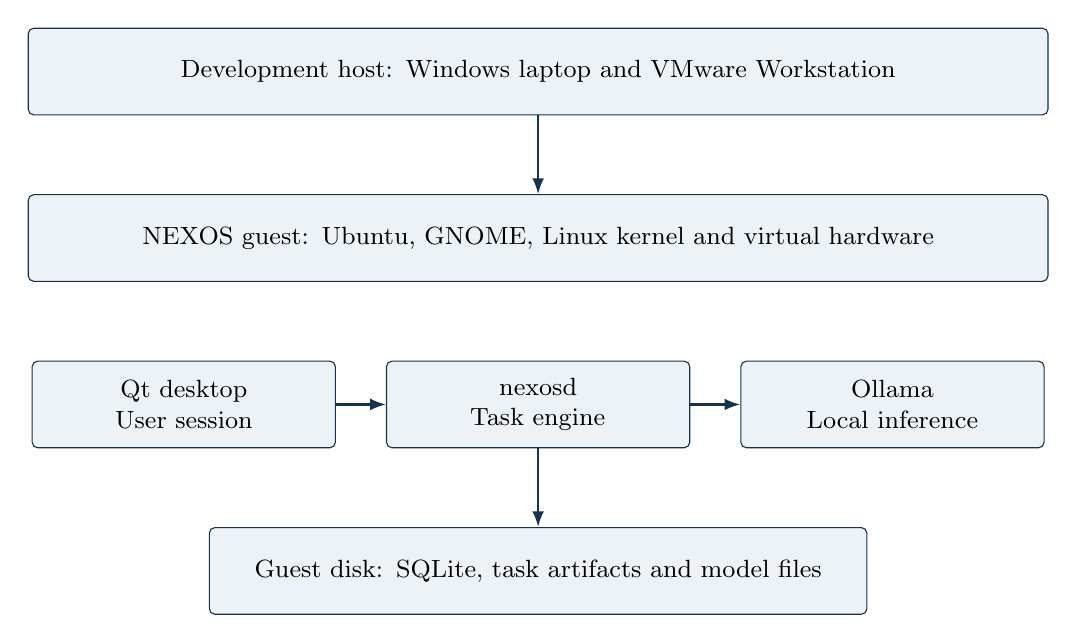
\begin{tikzpicture}[node distance=10mm]
\node[box,text width=126mm] (host) {Development host: Windows laptop and VMware Workstation};
\node[box,below=of host,text width=126mm] (guest) {NEXOS guest: Ubuntu, GNOME, Linux kernel and virtual hardware};
\node[box,below=of guest,xshift=-45mm,text width=35mm] (ui) {Qt desktop\\User session};
\node[box,below=of guest,text width=35mm] (engine) {nexosd\\Task engine};
\node[box,below=of guest,xshift=45mm,text width=35mm] (model) {Ollama\\Local inference};
\node[box,below=of engine,text width=80mm] (data) {Guest disk: SQLite, task artifacts and model files};
\draw[flow] (host)--(guest);
\draw[flow] (ui)--(engine);
\draw[flow] (engine)--(model);
\draw[flow] (engine)--(data);
\end{tikzpicture}
\caption{Proposed VMware deployment. Persistent application state belongs to the installed guest disk.}\label{fig:deployment}
\end{figure}

The daemon is proposed as a systemd user service so its lifecycle follows the relevant user session. Ollama uses a separate service identity and a local inference endpoint. An endpoint reachable by the user must not be exposed to the broader network by default. Local socket ownership and permissions protect ordinary cross user access; they are not a complete defense against a malicious process already running as the same desktop user.

An installed VM retains state after reboot. A live ISO session usually writes to a temporary overlay and may lose state when shut down. The interface must clearly identify this condition. Credential setup and important history should be associated with an installed persistent environment or a deliberately configured persistence mechanism.

\section{Data Flow and Trust Boundaries}
The principal input flows are the user's intent, selected project data, model proposals and tool observations. The principal output flows are action previews, task events, generated artifacts and verified result summaries. Data crossing from project content or a provider response into an action request must pass schema and policy checks.

\begin{figure}[htbp]\centering
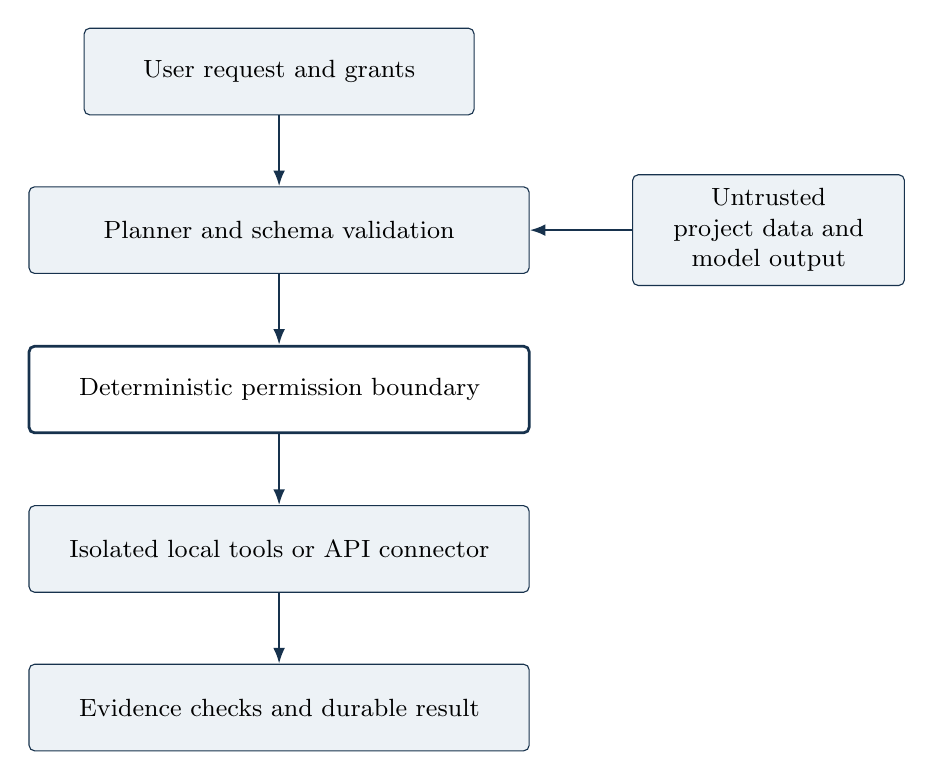
\begin{tikzpicture}[node distance=9mm]
\node[box,text width=46mm] (request) {User request and grants};
\node[box,below=of request,text width=60mm] (plan) {Planner and schema validation};
\node[box,right=13mm of plan,text width=31mm] (untrusted) {Untrusted project data and model output};
\node[box,below=of plan,text width=60mm,fill=white,line width=1pt] (broker) {Deterministic permission boundary};
\node[box,below=of broker,text width=60mm] (tools) {Isolated local tools or API connector};
\node[box,below=of tools,text width=60mm] (verify) {Evidence checks and durable result};
\draw[flow] (request)--(plan);
\draw[flow] (untrusted)--(plan);
\draw[flow] (plan)--(broker);
\draw[flow] (broker)--(tools);
\draw[flow] (tools)--(verify);
\end{tikzpicture}
\caption{Conceptual data flow. Untrusted content can inform a proposal but cannot grant execution authority.}\label{fig:dfd}
\end{figure}

The broker, adapter code, verifier, relevant database transitions and operating system mechanisms form the execution trusted computing base. Keeping this boundary small makes review more practical. The model is outside the authority boundary, even if it runs locally. A local model can still misunderstand a task or be influenced by hostile input.

\section{Architectural Alternatives}
A browser interface with a local HTTP service was considered earlier. The current design chooses Qt because the project goal is an integrated native workstation experience. Internal APIs remain necessary, but a public web server is not required. The selected socket transport also avoids making a local web origin part of the initial application boundary.

A large distributed stack with multiple databases and message brokers is unnecessary for the first single machine prototype. SQLite and a bounded Python engine reduce installation and recovery complexity. Framework based agent orchestration can be evaluated later against the explicit state machine, but framework adoption must demonstrate a concrete benefit and preserve the same authority rules.

A complete operating system written from scratch would consume the project effort in drivers, boot support and low level resource management. Reusing Ubuntu directs the work toward the research and engineering problem of agent execution. The distribution deliverable demonstrates integration of that work into an operating environment.

\chapter{Task Planning and Execution}
\section{Intent Resolution and Task Contracts}
A task begins with a goal and the resources to which that goal applies. For example, a diagnosis request needs a project root and an output directory. A meeting request additionally needs a calendar, start time, duration, timezone and attendees. The engine should resolve essential ambiguity before proposing a side effect. It should not guess an email address or silently interpret a relative date in an unknown timezone.

The proposed task contract contains a task identifier, goal, normalized inputs, capability references, deadline and budget. A model can help classify the request and suggest a supported workflow. The engine checks the result against a schema and rejects fields or tools that are not part of the contract. Bounded retries may repair formatting errors; they do not permit the model to invent new adapter capabilities.

\section{Plan Representation and Validation}
A plan is represented as a directed graph $G=(V,E)$ in which each node identifies a registered tool and each edge expresses a prerequisite. A step includes typed arguments, declared read and write resources, a timeout and required postconditions. An edge $u\rightarrow v$ means that step $v$ may start only after step $u$ completes according to its dependency policy.

For the prototype, the plan must be finite, acyclic and small enough for review. The current foundation accepts at most twelve steps and only three tool identifiers. The proposed planner may use a larger registry later, but limits should remain explicit. Validation rejects duplicate step identifiers, missing dependencies, unsupported tools and cycles before any action is dispatched.

Topological validation can be implemented with indegree counts and a ready queue. Its graph traversal cost is $O(|V|+|E|)$, excluding argument and policy checks. A valid graph is necessary but insufficient: a plan may still be semantically wrong, overbroad or unsupported by the user's intent. Those conditions require task checks, capability checks and outcome verification.

\section{Scheduling and Resource Admission}
The proposed scheduler admits a step when all required predecessors have succeeded, its resources are available and its execution budget remains valid. The initial policy favors simple FIFO ordering with a small concurrency limit. Later priority classes may distinguish interactive tasks from background indexing, with aging to prevent starvation.

Read operations on the same immutable snapshot can run concurrently. Conflicting writes require serialization or explicit locking. Locks should be acquired in a stable order to reduce deadlock risk. Model inference is separately queued because it may consume most of the guest's memory. Specialist roles do not justify loading several large models at once.

Cooperative preemption means pausing at documented safe boundaries or cancelling a worker and recording its observed state. It does not imply transparent suspension of arbitrary external effects. A remote event creation may complete even if the local request times out; that case requires reconciliation rather than an immediate duplicate retry.

\section{Task State Model}
The complete design uses states for intake, validation, planning, approval, execution, verification and terminal outcomes. A transition is recorded with its task identifier, timestamp and reason. The implemented foundation currently exercises a smaller path: received, planned, running, verifying and succeeded, with failed outcomes recorded on errors.

\reportfigure{nexos-task-workflow.png}{1}{Intended request, authorization, execution and verification workflow.}{fig:taskflow}

Waiting for approval is not the same as running. Cancellation requested is not the same as cancelled. A task with an unknown external effect should be marked for reconciliation rather than reported as a clean failure or success. These distinctions prevent a conversational summary from concealing an unresolved operation.

\section{Execution Algorithm}
The following pseudocode specifies the intended execution loop. It is an architectural algorithm; the current foundation implements a fixed diagnosis sequence rather than this complete concurrent scheduler.

\begin{lstlisting}[caption={Proposed bounded task execution algorithm}]
validate_task(task)
plan = propose_or_select_plan(task)
validate_schema_registry_and_dag(plan)
persist(plan, state="PLANNED")
while unfinished_steps(plan):
    enforce_task_budget(task)
    ready = dependency_ready_steps(plan)
    for step in admit_with_resource_limits(ready):
        action = normalize_action(step)
        decision = broker.authorize(action, task.grants)
        if decision.requires_approval:
            persist_waiting_and_present_preview(action)
            continue
        if not decision.allowed:
            fail_step_without_dispatch(step)
            continue
        record_attempt_before_dispatch(step)
        observation = execute_registered_adapter(action)
        evidence = verify_postconditions(step, observation)
        persist_attempt_and_evidence(step, evidence)
    if no_progress_possible():
        wait_for_decision_or_end_with_specific_reason()
return aggregate_verified_outcome(plan)
\end{lstlisting}

The record before dispatch narrows the uncertainty window after a crash. It does not create an atomic transaction across SQLite and an external provider. Each adapter therefore declares whether it is read only, idempotent, safely retryable or requires reconciliation. Retry policy is attached to the operation, not inferred from a generic HTTP error alone.

\section{Worked Diagnosis Workflow}
The user grants a project directory and requests a report. The file adapter identifies supported manifests within that root. The diagnostics adapter parses metadata without importing modules or running package scripts. The report adapter writes a new file in the granted output directory. The verifier reopens the report, checks its identity and digest, and confirms that source manifests have not changed during the operation.

A missing manifest produces a clear unsupported input result. Malformed JSON or TOML is reported as an input failure. An existing output filename is not overwritten by the current foundation. A source file changed during inspection causes verification failure, because the report would otherwise combine observations from different states. These outcomes are useful even without a model and establish a deterministic reference for later natural language requests.

\section{Worked Calendar Workflow}
The proposed connector normalizes the date and timezone, checks the selected calendar where authorization permits, and presents the exact event details. The user reviews the title, time, duration, attendees and notification behavior. The approved operation is executed through Google Calendar APIs, including conference data creation when supported by the account \cite{calendar}.

The connector stores a stable request identity for retry handling and reads back the event. It verifies the returned time interval, attendee list and conference state. If meeting link generation is still pending, the task remains incomplete until a bounded follow up check resolves it or a specific limitation is reported. The browser is not required merely to navigate to a search engine; a documented API is the preferred integration for this workflow.

\section{Verification and Partial Results}
Let $P_i$ denote the required postconditions for step $i$. A step succeeds only when each required predicate is satisfied by accepted evidence. The task outcome aggregates required step outcomes; optional outputs may be reported separately. An artifact's hash proves equality with expected bytes, not the truth of every statement in those bytes.

For this reason, NEXOS uses domain specific verifiers. A file move check compares source and destination state; a report check validates content and source provenance; a calendar check inspects provider state. Partial output can be preserved for diagnosis, but must be labeled with its failed or incomplete verification state. The user should never need to infer failure from an apparently successful final message.

\chapter{Security and Permission Design}
\section{Threat Model}
The main threats considered are malicious instructions embedded in project content, malformed model output, resource access outside the task scope, accidental overwrite, unauthorized network access, stale approvals and misleading success claims. The design also considers oversized inputs, runaway processes, credential leakage and duplicate remote writes after a timeout.

The prototype assumes a trustworthy host kernel, administrator and NEXOS installation. It does not claim to defeat a compromised root account or all attacks by an adversarial process already running as the same desktop user. Process separation alone does not create a strong same user security boundary. These assumptions must be stated so that test results are interpreted within a defined scope.

\section{Capabilities and Action Policy}
A capability identifies a permitted operation over a specific resource under explicit constraints. For example, a task may read selected manifests under one project root and create a new report under one output root. It does not thereby gain access to the entire home directory, cloud credentials or arbitrary shell execution.

The proposed authorization predicate is:
\begin{equation}
\begin{aligned}
\operatorname{allow}(a,C)={}&\operatorname{registered}(a)\land\operatorname{valid}(a)\\
&\land\operatorname{inScope}(a,C)\land\operatorname{policyOK}(a)\\
&\land\operatorname{grantValid}(a).
\end{aligned}
\end{equation}
Every term is checked by deterministic code. A model explanation cannot substitute for a missing term. Capabilities are narrowed to the tool, resource and lifetime needed for the task, and the adapter receives the resolved action rather than an unconstrained command string.

\begin{table}[htbp]\centering\small
\caption{Proposed action categories and default handling}
\begin{tabularx}{\textwidth}{P{18mm}Y Y}
\toprule\textbf{Class} & \textbf{Example} & \textbf{Default handling}\\\midrule
T0 & Explain an already available result & No new resource access\\
T1 & Read granted manifests; create a requested new report & Execute within the task's existing grants\\
T2 & Overwrite a file; send calendar invitations & Preview concrete effect and obtain matching approval\\
T3 & Arbitrary root command or unsupported privileged change & Deny in the initial prototype\\\bottomrule
\end{tabularx}\end{table}

These categories are project policy, not a universal security standard. A user's original request can already authorize an action when its effect is concrete and the policy permits it. Repeated approvals for the same unchanged authorized step would add friction without adding a new boundary. Materially changed destinations, recipients or destructive effects require a new decision.

\section{Approval Binding and Replay Prevention}
The planned approval record binds a task, tool version, canonical arguments, resource identities, expiry and nonce. A changed event time or file destination invalidates the earlier approval. The broker consumes a one use grant transactionally where required. The interface shows the same normalized parameters that the broker will authorize.

An in process approval object should not be described as cryptographically secure merely because it contains a hash. If signed or message authenticated grants are introduced, key custody, verification and replay behavior must be specified and tested. The current foundation has scoped file access but no cryptographic grant system.

\section{Filesystem Boundary}
The foundation validates the project and output roots, rejects unregistered filenames and checks for links in relevant paths. Manifest reads are bounded to 128 KiB and report writes to 512 KiB. New report files use exclusive creation so an existing file is not silently replaced. These checks are useful application controls for the fixed workflow.

There remains a gap between path validation and use if another process can mutate the filesystem concurrently. The later Linux adapter design should use descriptor relative operations, avoid following links and validate the actual opened resource. Sandbox mounts should expose only the necessary roots. Race resistance must be tested directly; passing a static symlink test is not proof of complete resistance to concurrent path replacement.

\section{Worker Isolation}
Bubblewrap will be used to construct a restricted filesystem and namespace environment for suitable tools. A local diagnostics profile should expose required runtime libraries read only, mount the selected project read only, provide a dedicated output directory and use temporary storage for scratch data. Network access is denied for tools that do not need it. Environment variables and inherited file descriptors must be minimized.

The profile must also consider process lifetime, writable locations, IPC exposure and device access. Resource limits are proposed through tested systemd settings or other verified process controls. Availability of a setting in documentation is not proof that it is enforced in the chosen user session or kernel configuration. A failed isolation preflight should stop the affected adapter instead of silently falling back to unrestricted execution.

\section{Prompt Injection Handling}
Repository files, fetched pages, tool responses and retrieved memory are data channels. Instructions contained in those sources do not supersede the user's task or grant new authority. The planner receives source labels and limited context, while the execution layer independently checks every proposed action.

The current foundation does not read arbitrary project README instructions or execute package scripts, so its tests can establish that those inputs do not affect its static workflow. A model integrated system will have a larger attack surface. Its evaluation should include malicious text that asks for secret access, new destinations, tool substitution and false completion. The goal is measured resistance within the supported tasks, not a claim of absolute prompt injection immunity.

\section{Secrets and Network Connectors}
OAuth refresh tokens and optional model provider keys belong in a credential store such as the Linux Secret Service. The database stores opaque credential references. Tokens should never be inserted into model prompts, report artifacts or ordinary event logs. A connector receives the minimum account access needed for its operation and handles revocation explicitly.

A browser fallback, if added later, requires a separately reviewed profile and session policy. Browser automation can expose cookies, pages and downloads that have broader effects than a single API call. It should not be treated as a generic escape hatch when a typed connector fails.

\section{Auditing and Residual Risk}
The current SQLite journal records task events but is not hash chained. A future audit chain may compute $h_i=H(h_{i-1}\Vert\operatorname{canonical}(e_i))$, where $e_i$ is an event. This can reveal changes relative to a trusted checkpoint. An attacker able to rewrite the entire database and checkpoint may recompute the chain, so local hashing alone is not strong nonrepudiation or proof of a correct action.

Security evidence must include denied access tests, resource limit tests, approval mismatch tests and secret redaction checks. Residual risks include model misunderstanding within an allowed scope, adapter defects, platform vulnerabilities and external service behavior. The release report should record these limits alongside successful tests.

\chapter{Data Management and Memory}
\section{Persistence Objectives}
Persistent state allows the engine to explain what happened, identify unfinished work and retain evidence after the interface closes. It must distinguish the task definition from its execution attempts. A retry is a new attempt with a relationship to the same step, rather than an overwrite that hides the earlier failure.

SQLite is selected for the initial single machine deployment because it provides transactions and a local file based database with a small operational footprint. The database schema and migration version are part of the application release. A schema upgrade should be tested against a backup of representative state and should fail visibly when incompatible data is encountered.

\section{Proposed Data Model}
\begin{figure}[htbp]\centering
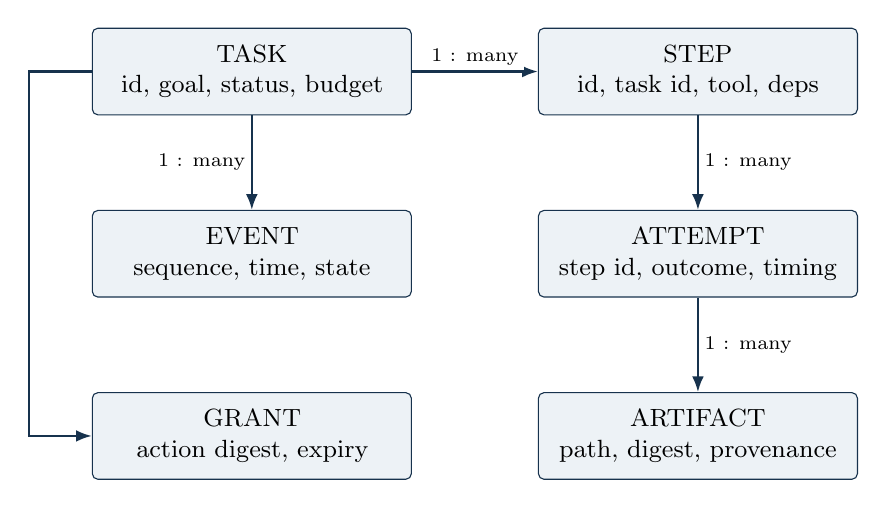
\begin{tikzpicture}[node distance=12mm]
\node[box,text width=37mm] (task) {TASK\\id, goal, status, budget};
\node[box,right=16mm of task,text width=37mm] (step) {STEP\\id, task id, tool, deps};
\node[box,below=of task,text width=37mm] (event) {EVENT\\sequence, time, state};
\node[box,below=of step,text width=37mm] (attempt) {ATTEMPT\\step id, outcome, timing};
\node[box,below=of event,text width=37mm] (grant) {GRANT\\action digest, expiry};
\node[box,below=of attempt,text width=37mm] (artifact) {ARTIFACT\\path, digest, provenance};
\draw[flow] (task)--node[labeltext,above]{1 : many}(step);
\draw[flow] (task)--node[labeltext,left]{1 : many}(event);
\draw[flow] (step)--node[labeltext,right]{1 : many}(attempt);
\draw[flow] (attempt)--node[labeltext,right]{1 : many}(artifact);
\draw[flow] (task.west)--++(-8mm,0)|-(grant.west);
\end{tikzpicture}
\caption{Proposed logical data model. The foundation currently implements task and event records, not every entity shown.}\label{fig:data}
\end{figure}

Task records hold the normalized request, current status and configuration identity. Step records hold tool versions, dependencies and declared resources. Attempt records hold dispatch and completion information. Events describe transitions and observations in order. Artifacts identify outputs and their digests; they do not require placing every large output directly inside SQLite. Approval records bind concrete actions to user decisions.

An evidence path must be resolved under an application controlled artifact root or explicitly granted destination. A database entry alone is not sufficient proof that a file still exists or has remained unchanged. The result viewer should check artifact availability and flag a digest mismatch rather than silently showing stale evidence as current.

\section{Four Memory Roles}
\textbf{Working memory} is the active context for a task: normalized inputs, recent observations and the current plan. It is bounded by a context budget and should not accumulate entire repositories.

\textbf{Episodic memory} records past tasks, attempts and outcomes. It supports history, debugging and later comparison of recurring failures. A short summary should link to the original evidence instead of replacing it.

\textbf{Semantic memory} is searchable information about granted projects and documents. Initially, FTS5 supplies token based text retrieval. Semantic vector similarity would require an embedding model, vector representation and a retrieval implementation; it is not provided merely by enabling FTS5.

\textbf{Procedural memory} contains reviewed reusable workflows, tool templates and applicable preconditions. A successful one time sequence becomes reusable only after its assumptions are made explicit. A remembered command must still be registered, authorized and verified when used again.

\section{Indexing and Provenance}
The proposed indexer enumerates only selected roots, applies file type and size limits, and stores source identifiers with modification times and content digests. Each chunk should carry enough provenance to locate the original material. Index updates should be incremental so a small change does not require processing the complete workspace.

Retrieval filters by current capabilities before returning content to the model. Revoking a root should remove or disable its derived entries, including summaries and embeddings if present. A retrieved result is quoted or summarized as source material and never treated as a privileged instruction. These rules prevent a useful memory feature from becoming an unintended route around resource permissions.

\section{Recovery Semantics}
When the daemon restarts, it reads incomplete attempts and classifies them by adapter behavior. Read only work can often be repeated. A file creation can be reconciled by checking its recorded destination and identity. A remote write may require a provider lookup using the stored request identifier. If its outcome cannot be determined, the task enters a needs attention state.

The database transaction that records an attempt cannot atomically commit an external service action. The design therefore aims for explicit reconciliation and controlled retries, not a universal exactly once guarantee. Each adapter documents its retry contract and duplicate prevention strategy. Crash injection tests must cover the intervals before dispatch, after dispatch and before persistence of the result.

\section{Retention and Backup}
Task history and artifacts should have configurable retention rules, with an option to preserve selected reports. Deleting a task should account for related summaries and retrieval entries, while avoiding deletion of user files merely referenced by the task. Backups should use a consistent database snapshot and include required artifact metadata.

The initial project does not require cloud synchronization. Introducing synchronization would add identity, conflict resolution and credential protection requirements. Keeping storage local reduces the first release's operational scope and makes the evaluation easier to reproduce.

\chapter{Desktop Interface and Workflows}
\section{Interaction Design}
The native assistant should make the task's state understandable at a glance. The main workspace combines a request area, current plan, progress timeline and result evidence. Navigation exposes task history, granted folders and configured connections. The user should be able to inspect what the system intends to do without reading raw internal protocol messages.

The interface must distinguish planning, waiting for a decision, execution and verification. A progress animation cannot imply a percentage when the amount of remaining work is unknown. Status labels such as ``Inspecting manifests'' or ``Checking the saved report'' are more useful than unsupported precision. Errors should identify the affected step and the action the user can take.

\section{Proposed Task Workspace}
Figure~\ref{fig:ui-task} is an interface concept for the planned Qt application. It shows an explicitly granted project and a report task with evidence links. The example data is illustrative. It is not a screenshot of a completed NEXOS desktop.

\reportfigure{ui-task-workspace.png}{1}{Proposed Qt task workspace showing scope, execution stages and evidence. Interface concept, not an implemented screen.}{fig:ui-task}

The request composer is accompanied by a visible scope indicator. The plan identifies meaningful actions rather than presenting a long conversation as the only record of work. A result view links to the report and shows which checks passed. If a source changes during execution, the evidence panel should state that verification failed instead of retaining a generic green completion indicator.

Keyboard navigation, visible focus and readable text are required. Controls need descriptive labels. Status must remain understandable in grayscale and should not depend solely on color. The Qt implementation should use appropriate accessibility properties and should be tested with keyboard only operation and enlarged text.

\section{Action Preview and Approval}
The approval view presents the concrete effect of a sensitive action. For a calendar request, it includes the selected account, calendar, normalized date and timezone, duration, attendee addresses and notification behavior. For a file change, it includes the destination, overwrite status and a diff or summary of the proposed change.

\reportfigure{ui-action-preview.png}{1}{Proposed calendar action preview with explicit details and a bounded approval choice. Illustrative data only.}{fig:ui-approval}

The interface binds the displayed preview to the action identifier that the broker will execute. If the engine revises an action, the old approval is invalidated and the changed details are shown. Approval and cancellation controls should have clear, distinct wording. The interface must not preapprove an action because a timer expired or because the model predicts that the user would agree.

\section{Use Case Specifications}
\subsection{Inspect a Project}
The actor is the logged in user. Preconditions are an available project root, an approved output directory and supported manifest files. The normal flow reads manifests, summarizes declared metadata, creates a new report and verifies its identity and source digests. The postcondition is a verified report with a persistent task record. Invalid syntax, unsupported input and changed source content are alternative outcomes.

\subsection{Perform a Reversible File Operation}
This planned workflow selects files within a granted root and previews destinations. The adapter rejects path escape, unexpected links and destination conflicts according to policy. A reversible operation records enough original state to support a documented undo action. Undo is a separate checked operation, not a promise that any arbitrary change can always be reversed.

\subsection{Schedule a Project Review}
This planned workflow requires a connected Google account and the relevant calendar authorization. The user supplies or confirms attendees, date, time, timezone and duration. The connector creates the approved event and checks the returned state. Provider denial, unavailable conferencing and ambiguous timeout outcomes are shown explicitly. The displayed meeting link is taken from verified provider data rather than generated by the model.

\section{First Run Experience}
First run setup should explain whether the user is in a temporary live session or an installed environment. It checks the engine, tool profiles, available storage and model readiness. The user chooses a local model configuration or an optional remote provider and grants a demonstration folder. The first task uses a prepared fixture so that the expected output is known.

The Core ISO includes the inference runtime but may need a model download before AI requests are available. The offline demonstration variant includes a selected model after licensing and resource checks. Local offline readiness must not be confused with external service readiness; a calendar connector still needs network access and account authorization.

\section{History and Failure Presentation}
The history view groups the request, plan version, attempts, approvals and evidence. A failed attempt remains visible even if a later retry succeeds. Users should be able to open a concise technical explanation without being forced to read every log line. Exported evidence should redact credentials and unnecessary private content.

Cancellation feedback must distinguish a stopped local worker from an external action whose status is still being reconciled. When work remains uncertain, the interface should say so directly. Clear incomplete states are part of trustworthy automation and are preferable to an unsupported success message.

\chapter{Implementation and Current Progress}
\section{Development Strategy}
Implementation begins with a deterministic workflow so that the execution path can be tested before model variability is introduced. The model will later select or propose actions using the same contracts. This provides a reference behavior for diagnosis tasks and makes it easier to separate planner failures from adapter or verification failures.

The current foundation is a Python package with a command line interface. It uses the standard library for JSON, TOML, SQLite, hashing and filesystem operations. Pydantic, the Qt interface and the inference gateway belong to later integration work. The package's small dependency set is intentional at this checkpoint and should not be mistaken for the dependency set of the final distribution.

\section{Implemented Module Structure}
\begin{table}[htbp]\centering\small
\caption{Implemented foundation modules}
\begin{tabularx}{\textwidth}{P{36mm}Y}
\toprule\textbf{Module or helper} & \textbf{Implemented responsibility}\\\midrule
\texttt{policy.py} & Scoped manifest reads, link checks, size limits and exclusive report creation.\\
\texttt{plan.py} & Fixed tool registry, dependency validation and bounded plan ordering.\\
\texttt{diagnosis.py} & Static parsing, report creation and evidence verification.\\
\texttt{journal.py} & Task and event persistence in SQLite.\\
\texttt{cli.py} & Diagnosis command, readiness report and structured error output.\\
\texttt{test\_foundation.py} & Ten tests for the supported workflow and adverse inputs.\\
Package helpers & Build a Debian archive and smoke test its extracted launcher.\\\bottomrule
\end{tabularx}\end{table}

The command line entry point accepts a project root, an output directory and a state database path. It returns a structured result including the task status, report path, report digest, findings and verification flags. The readiness command reports platform and tool availability. Tool discovery is a preflight observation; it is not proof that a complete ISO build will succeed.

\section{Static Diagnosis Behavior}
The foundation recognizes \texttt{pyproject.toml}, \texttt{requirements.txt} and \texttt{package.json}. It parses declared metadata and records a digest for each inspected source. For Python project metadata, it counts declared dependency entries. For Node metadata, it combines dependency and development dependency keys. For requirements files, it counts nonempty, noncomment entries, including directives; it does not claim that each entry names a resolved installed package.

The workflow does not import project modules, run installation hooks or execute scripts. It therefore cannot establish that the application starts, that dependencies are installed or that a runtime version is compatible. Those checks require later Linux adapters and distinct evidence. The report explicitly labels its scope as static manifest inspection.

\section{Verification Implementation}
The report verifier reopens the generated file and compares its digest with the bytes produced by the report adapter. It checks the task identity and required findings, then rereads supported source manifests and compares their digests with those recorded during inspection. A changed report or source causes an error instead of success.

This is independent deterministic checking of the output path within the current application, not isolation of a verifier into a separate security domain. A compromised process with equivalent authority remains outside the foundation's demonstrated protection. The distinction matters when explaining what a successful unit test proves.

\section{Observed Foundation Results}
The development checkpoint recorded on 19 October 2026 contains ten passing foundation tests on Windows with Python 3.12.14 and Ubuntu WSL with Python 3.12.3. The tests cover successful and failed task records, path escape, overwrite refusal, ignored README instructions and package scripts, oversized input, invalid plans, source changes, report tampering and symlink denial.

These tests exercise a fixed workflow. They do not measure natural language task accuracy, Linux sandbox escape resistance, complete same user isolation, crash recovery of remote operations or ISO installation reliability. Those results remain to be collected using the evaluation protocol in Chapter~\ref{ch:evaluation}.

\begin{table}[htbp]\centering\small
\caption{Implementation status at the report checkpoint}
\begin{tabularx}{\textwidth}{Y P{31mm}Y}
\toprule\textbf{Capability} & \textbf{Status} & \textbf{Evidence or next gate}\\\midrule
Static manifest diagnosis & Implemented & Fixed workflow and tests\\
Scoped report access & Implemented foundation & Adverse path and overwrite checks\\
SQLite task records & Implemented foundation & Transition persistence tests\\
Debian foundation archive & Built and checked & Extraction smoke test\\
Model driven plans & Planned & Gateway and schema tests\\
Linux worker sandbox & Planned & Profile and denial tests\\
Native Qt application & Planned & Desktop workflow tests\\
Calendar connector & Planned & Sandbox account integration tests\\
Bootable NEXOS ISO & Planned & Live and installed VM qualification\\\bottomrule
\end{tabularx}\end{table}

\section{Foundation Package}
The package \texttt{nexos-engine-foundation} version 0.1.0 has been built as an architecture independent Debian archive. It installs the Python foundation and a launcher and declares its Python dependency. A smoke test checks the archive digest, extracts its contents into a temporary directory, invokes the packaged version and runs the fixture workflow.

Extraction testing avoids confusing a valid archive with a qualified system installation. Clean install, upgrade, removal, desktop registration and service lifecycle tests are still required for final packages. The foundation archive does not contain a model, full desktop interface or complete operating system.

\section{Reproducible Commands}
The following commands describe the current source workflow on a suitable Python 3.12 environment. The bundled example is static metadata and does not need dependency installation.
\begin{lstlisting}[caption={Current foundation workflow}]
python3 tools/run_nexos.py doctor --workspace .
python3 tools/run_nexos.py diagnose \
  --project examples/demo-project \
  --output .nexos/reports \
  --state .nexos/state.sqlite3
python3 -m unittest discover -s tests -v

# On a qualified Linux environment with dpkg-deb:
python3 tools/build_foundation_deb.py
python3 tools/check_foundation_package.py
\end{lstlisting}

Results should be saved with the source revision and environment details. A repeat run may create a different task identifier and report filename while preserving the expected semantic findings. Reproducibility therefore compares specified properties and recorded inputs, rather than assuming every generated byte is identical.

\chapter{Packaging and ISO Delivery}
\section{Delivery Artifacts}
The required release artifact is a customized bootable Ubuntu ISO. Application packages are the building blocks used to assemble and update that image. A prebuilt virtual machine is an optional convenience artifact produced from a tested installation. These formats have different purposes: an ISO boots installation or live media, whereas a VM export includes an installed virtual disk and configuration.

The proposed Core ISO contains Ubuntu, desktop integration, the NEXOS interface and engine, an inference runtime and first run configuration. It may require a model download before AI inference is ready. An Offline Demo ISO additionally contains one tested model and prepared local fixtures after redistribution terms are checked. Neither variant makes internet dependent services operate offline.

\reportfigure{nexos-iso-pipeline.png}{1}{Proposed package to ISO pipeline with clean virtual machine qualification.}{fig:iso}

\section{Package Boundaries}
The final package organization should separate the engine, native desktop and distribution integration where doing so improves upgrade and dependency management. The engine package provides task logic and the user service. The desktop package provides Qt resources and application launch metadata. Integration assets provide defaults, first run setup and the selected tool profiles. Model weights have their own size, version and licensing considerations and should not be hidden inside an undocumented application dependency.

Each package needs a version, dependency specification, file manifest, license information and installation behavior. Package scripts must be narrowly scoped and should not embed developer credentials or create globally permissive access. Installation should be tested on a clean guest, including service startup, removal and a controlled upgrade from the previous supported state.

\section{Base Image and Build Inputs}
The project selects an Ubuntu 24.04 LTS desktop image for the target architecture. Before customization, the complete downloaded file is checked against its published digest, and the checksum signature is authenticated using an appropriate trusted Ubuntu signing key. Candidate metadata in a JSON file is not equivalent to a verified download.

The build record includes the exact image filename and digest, package versions, NEXOS revision, model identifier and digest where applicable, customization scripts and tool versions. Changes in the upstream base should be deliberate and recorded. Reproducible inputs improve traceability even when the build has not yet achieved byte identical reproducibility.

\section{Customization Workflow}
Cubic provides a practical initial workflow for customizing Ubuntu based live images \cite{cubic}. The project should preserve package lists and overlay files outside the interactive build session so that changes are reviewable. The customized filesystem incorporates qualified NEXOS packages, desktop launchers, service units and demonstration fixtures.

The image must preserve a valid inherited boot and installer structure. Repacking a filesystem into an arbitrary archive does not create a qualified bootable distribution. After image assembly, a new VM tests the live session, installer and installed system. A successful build command is only the beginning of distribution qualification.

\section{Build Environment and Storage}
The existing Ubuntu WSL environment has supported Python tests and Debian archive creation. At the recorded preflight, \texttt{dpkg-deb} and \texttt{mksquashfs} were found, while \texttt{cubic}, \texttt{xorriso} and \texttt{bwrap} were not found in its executable search path. This makes it useful for foundation work, but it has not yet been qualified as the full desktop image builder.

A tested Ubuntu desktop VM is the primary fallback for Cubic and image assembly. Its build directory and virtual disk should be placed on a volume with sufficient free space. Disk planning must include temporary extraction, caches, resulting ISO and test installation, not just the final download size. Snapshots and model copies can grow unexpectedly and should be tracked explicitly.

\section{Boot and Installation Qualification}
\begin{figure}[htbp]\centering
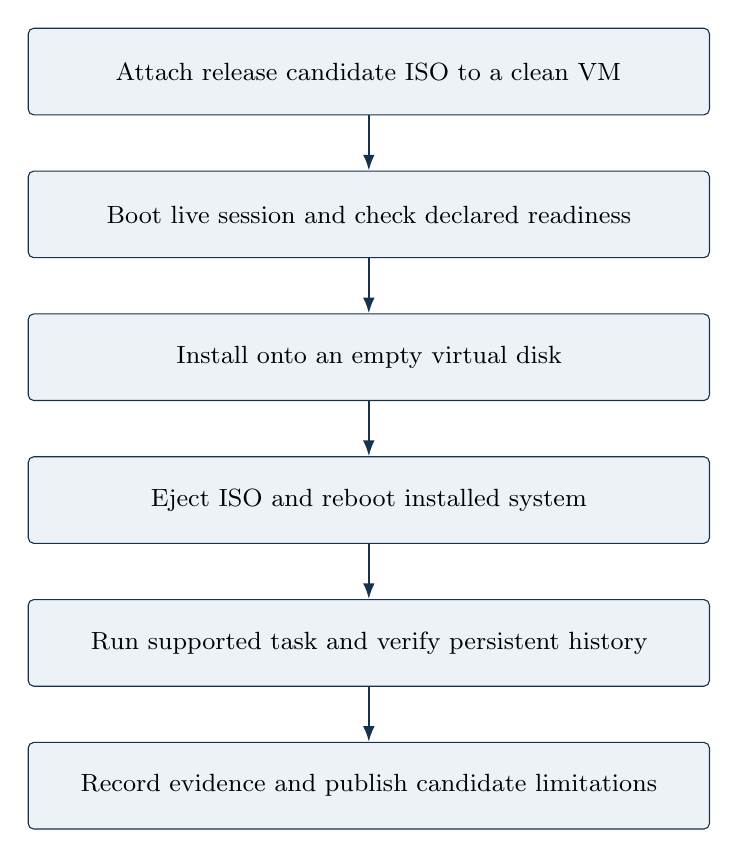
\begin{tikzpicture}[node distance=7mm]
\node[box,text width=83mm] (a) {Attach release candidate ISO to a clean VM};
\node[box,below=of a,text width=83mm] (b) {Boot live session and check declared readiness};
\node[box,below=of b,text width=83mm] (c) {Install onto an empty virtual disk};
\node[box,below=of c,text width=83mm] (d) {Eject ISO and reboot installed system};
\node[box,below=of d,text width=83mm] (e) {Run supported task and verify persistent history};
\node[box,below=of e,text width=83mm] (f) {Record evidence and publish candidate limitations};
\draw[flow] (a)--(b);\draw[flow] (b)--(c);\draw[flow] (c)--(d);\draw[flow] (d)--(e);\draw[flow] (e)--(f);
\end{tikzpicture}
\caption{Proposed release qualification sequence. Booting the installer alone does not qualify the installed product.}\label{fig:boot}
\end{figure}

The first compatibility target is x86\_64 VMware Workstation with UEFI and Secure Boot disabled for the prototype. Exact host, hypervisor and virtual hardware versions must be recorded. Support for other hypervisors, Secure Boot or physical computers requires separate tests. The release must not promise operation on every VMware version or device.

The installed system is rebooted after ejecting the ISO so that accidental reliance on live media is detected. Tests inspect the desktop, daemon, model readiness, granted tools and stored artifacts. An offline variant is tested with networking disconnected for its declared local tasks. Network connectors are tested separately with controlled accounts and fixtures.

\section{Release Hygiene and Updates}
Before release, the image is checked for developer tokens, shell history, private documents, cached account sessions and machine specific identifiers. A prebuilt VM requires additional sanitization because it has already completed installation and may contain user state. A release manifest records checksums, component versions, known limitations and the test environment.

Updates should preserve the user's task history and selected settings through explicit migration behavior. Model updates are evaluated as changes to the system, because planning quality and resource use can change. Rollback instructions must state which state formats remain compatible; restoring an old package does not automatically reverse a database migration.

\section{When ISO Work Begins}
Software development and image input preparation can proceed now. An early boot prototype is useful after the base image and builder are qualified, even if it contains only a clearly labeled foundation package. The complete release image should be assembled after the engine, interface and service packages work on a clean Ubuntu installation.

This order avoids treating packaging as a substitute for working software while still identifying boot and installer issues early. At the report checkpoint, the foundation Debian archive exists; a bootable NEXOS release ISO has not been produced.

\chapter{Testing and Evaluation}\label{ch:evaluation}
\section{Evaluation Questions}
The evaluation asks whether NEXOS completes supported tasks, respects granted resources, detects incorrect outcomes and recovers predictably from interruption. It also asks whether the selected model and runtime configuration are practical on the available hardware. These questions require separate measurements; a single success percentage cannot describe all of them.

The experiment must distinguish deterministic foundation behavior from model driven behavior. It must also distinguish a source checkout from an installed package and a complete ISO. A feature is accepted at the layer where it will be used, with evidence recorded for that environment.

\section{Fixture Design}
Each fixture contains a known initial state, a task description, allowed resources, expected postconditions and a reset procedure. Static diagnosis fixtures include valid Python metadata, valid Node metadata, missing manifests, malformed documents, oversized input, changed source content and destination conflicts. Permission fixtures include attempted path traversal, linked resources and unsupported tools.

Later agent fixtures introduce ambiguous project names, hostile instructions in source content, unknown tools and model output that violates the schema. Connector fixtures use test accounts and controlled recipients. Release fixtures begin from an empty virtual disk so that dependencies inherited from a developer environment do not conceal packaging problems.

The proposed first evaluation suite contains approximately forty task scenarios, grouped by workflow and failure mode. This is a planning target, not a completed dataset. A pilot should determine whether the scenarios are sufficiently distinct and whether each oracle is correct before the final count is frozen.

\section{Metrics}
Verified task success is defined as:
\begin{equation}
\operatorname{VSR}=\frac{\text{tasks satisfying all required postconditions}}{\text{attempted tasks}}.
\end{equation}
Permission violation rate is the fraction of evaluated attempts that produce an effect outside their granted scope. A violation counts even when the intended task also succeeds. False success rate is the fraction of tasks reported successful whose independent evaluation oracle fails.

Latency should be reported as median and tail values with sample counts. Separate planning time, tool execution time and verification time when practical. Resource observations include peak resident memory, guest memory pressure, model load time and disk consumption. Human intervention counts record clarification, approval and manual repair separately.

\begin{table}[htbp]\centering\small
\caption{Planned metrics and evidence collection}
\begin{tabularx}{\textwidth}{P{34mm}Y Y}
\toprule\textbf{Metric} & \textbf{Collected evidence} & \textbf{Interpretation}\\\midrule
Verified success & Oracle result and task status & Supported task completion\\
False success & Claimed success with failed oracle & Misleading completion behavior\\
Permission violation & Forbidden filesystem or API effects & Boundary failure\\
Latency & Timed stages and total duration & Interactive performance\\
Memory use & Peak process and guest observations & Hardware feasibility\\
Recovery outcome & Crash point and reconciled state & Durable workflow behavior\\
Installation outcome & Live, install and reboot evidence & Distribution readiness\\\bottomrule
\end{tabularx}\end{table}

\section{Baselines and Experimental Controls}
The deterministic diagnosis CLI is a baseline for tasks already covered by its fixed plan. A manual workflow can provide a time and interaction comparison if the task and participant procedure are documented. A model based planner is evaluated using the same fixtures and allowed tool set. An optional ablation can compare verification enabled and disabled in an isolated test harness, without exposing a user workstation to unchecked actions.

The experiment records the model identifier, digest or immutable version where available, quantization, context settings, generation parameters, inference runtime and tool versions. Model dependent tasks should have repeated trials because their outputs may vary. A practical initial choice is three trials per scenario, followed by more trials when variance or failures require investigation. This is a proposed procedure, not an assurance of statistical power.

Task splits should prevent a held out evaluation from being tuned repeatedly after observing its answers. If prompt or adapter changes are made after failures, the report should distinguish development fixtures from the final evaluation run. Results are reported per task family as well as in aggregate to avoid hiding a weak workflow behind many easy cases.

\section{Foundation Test Evidence}
\begin{longtable}{P{17mm}P{87mm}P{34mm}}
\caption{Recorded foundation test coverage}\\
\toprule\textbf{Test} & \textbf{Checked behavior} & \textbf{Recorded result}\\\midrule\endfirsthead
\toprule\textbf{Test} & \textbf{Checked behavior} & \textbf{Recorded result}\\\midrule\endhead
F01 & Verified success and persisted transition sequence & Passed\\
F02 & Malformed manifest produces failed status & Passed\\
F03 & Traversal and unregistered reads are rejected & Passed\\
F04 & Output escape and overwrite are refused & Passed\\
F05 & README instructions and package scripts are not executed & Passed\\
F06 & Report tampering is detected & Passed\\
F07 & Changed source is detected during verification & Passed\\
F08 & Oversized manifest is rejected & Passed\\
F09 & Unknown tools, missing dependencies and cycles are rejected & Passed\\
F10 & Symlinked manifest access is rejected & Passed\\\bottomrule
\end{longtable}

The recorded checkpoint contains ten passing tests on each of the two development environments. This is test coverage of the current implementation, not a measured 100 percent agent success rate. No model participated in those tests. The package extraction smoke test is additional evidence that the foundation launcher and fixture work from the built archive, but it does not qualify installation or the complete distribution.

\section{Fault Injection and Adversarial Tests}
Fault injection will terminate the engine at defined points and then examine recovery. Candidate points include after recording a step, after a file is created and after a remote provider accepts a write but before the response is persisted. The expected behavior is a correctly classified state with no blind duplicate operation.

Security tests will attempt unauthorized file reads, unexpected writes, network use from offline profiles, stale grant reuse and substitution of approved parameters. Prompt injection tests will place hostile instructions in project documents and tool outputs. Tests should inspect the actual environment for effects; a denied message alone is insufficient if a forbidden action occurred first.

\section{Acceptance Gates}
The foundation gate requires passing functional and adverse input tests. The Linux boundary gate requires demonstrated mount, network and process limits for each enabled profile. The model gate requires valid plans and measured task behavior under the selected inference settings. The desktop gate requires visible progress, approval binding and cancellation handling. The distribution gate requires clean installation and persistent reboot checks.

No numerical performance target is presented as achieved. The project may choose an acceptance threshold after a pilot establishes realistic performance, but it must publish the threshold before the final evaluation and report all exclusions. Any observed permission violation or false success requires investigation before the affected workflow is represented as qualified.

\section{Threats to Validity}
A small fixture suite may overrepresent familiar tasks. Synthetic projects may omit real world edge cases. Different hardware and model settings may change latency substantially. Manual comparisons can be biased by participant familiarity. A verifier can itself contain defects, and a local test environment may not reproduce external service failures.

Mitigation includes held out scenarios, explicit reset procedures, independent oracle review, multiple trials and publication of environment details. Conclusions should remain limited to the tested scope. The report should state unresolved failures rather than removing difficult cases without explanation.

\chapter{Development Roadmap and Conclusion}
\section{Phased Methodology}
The project uses staged implementation with an acceptance gate after each major layer. A deterministic reference workflow precedes model integration. Linux isolation precedes broader execution. Native interface and service integration precede release packaging. Image prototyping can proceed in parallel with software development once its inputs are qualified, but final release depends on both paths.

The following sixteen week plan is a relative planning baseline. It is not a confirmed academic deadline. The team should map it to the department calendar and revise estimates after the first Linux and model integration tasks.

\begin{table}[htbp]\centering\small
\caption{Proposed development phases and completion gates}
\begin{tabularx}{\textwidth}{P{19mm}Y Y}
\toprule\textbf{Weeks} & \textbf{Main work} & \textbf{Completion gate}\\\midrule
1 to 2 & Foundation contracts, fixtures and static workflow & Deterministic tests and evidence\\
3 to 4 & Broker, Linux profiles and resource limits & Boundary tests on target Linux\\
5 to 6 & Ollama gateway and structured planning & Valid plans and measured model settings\\
7 to 8 & Scheduling, cancellation and recovery & Fault injection and reconciliation\\
9 to 10 & Native Qt interface and user service & Complete desktop workflow\\
11 to 12 & Scoped retrieval and calendar connector & Account and approval tests\\
13 to 14 & Packages and ISO integration & Clean live and installed guest\\
15 to 16 & Evaluation, corrections and report finalization & Reproducible evidence and limitations\\\bottomrule
\end{tabularx}\end{table}

\section{Team Workstreams}
Four workstreams fit the four member team: execution and permissions; model integration and memory; native interface and workflows; and packaging, evaluation and documentation. These are proposed responsibilities, not claims about individual contributions already completed. Members should rotate review responsibilities so that critical adapters and verifiers are inspected by someone other than their original author.

Shared contracts should be agreed before parallel implementation. The interface and engine need a stable message schema; the scheduler and adapters need consistent failure semantics; the evaluator needs fixture reset rules. A weekly integration checkpoint should run the supported workflow from a clean checkout and record unresolved dependencies.

\section{Risk Register}
\begin{longtable}{P{34mm}P{53mm}P{51mm}}
\caption{Project risks and mitigation actions}\\
\toprule\textbf{Risk} & \textbf{Potential consequence} & \textbf{Mitigation}\\\midrule\endfirsthead
\toprule\textbf{Risk} & \textbf{Potential consequence} & \textbf{Mitigation}\\\midrule\endhead
Model memory pressure & Slow or unresponsive guest & Small measured model, bounded context and serial inference\\
Invalid model plans & Failed or unsafe proposals & Registry and schema checks before dispatch\\
Incomplete sandbox profile & Access beyond intended resources & Fail closed preflight and direct denial tests\\
Insufficient build storage & Interrupted image creation & Track temporary use and limit snapshots\\
External API changes & Connector failure & Isolated adapter and recorded API behavior\\
Ambiguous remote timeout & Duplicate or unknown event & Stable request identity and reconciliation\\
Overextended scope & Incomplete final integration & Prioritize a few end to end workflows\\
Unqualified packaging & Works only on developer machine & Clean guest install and reboot tests\\
Misstated results & Invalid academic conclusions & Separate implemented, proposed and measured claims\\\bottomrule
\end{longtable}

\section{Prioritized Extensions}
The most useful near term additions are action previews, reversible file workflows, saved routines and searchable execution evidence. These features improve control and reuse without requiring unrestricted automation. Saved routines should reference reviewed templates and current grants. A schedule triggers a task under a defined policy; it should not preserve a broad authorization indefinitely.

Semantic retrieval can follow reliable keyword search, with evaluation of relevance, provenance and revocation. Voice and multilingual input can broaden accessibility once the text workflow is stable. Speech recognition introduces its own ambiguity, so sensitive names, destinations and times still need clear confirmation in the interface.

Later extensions include additional application connectors, a reviewed plugin system, bounded visual automation and optional remote model providers. A plugin system requires versioned contracts, dependency management, isolation and a qualification process. More autonomy should be introduced only when the relevant operations have adequate verification and recovery behavior.

\section{Expected Outcomes}
The intended final outcomes are a native assistant, a local execution engine, a qualified set of adapters, a persistent evidence store, an evaluated task suite and a bootable ISO. The final report should include measured results for the exact release candidate and document unsupported cases. The present foundation establishes only the first deterministic workflow and its package checkpoint.

The project is valuable if a reviewer can reproduce a supported request, observe how authority is checked, inspect the resulting evidence and repeat the workflow from a clean installation. This is a stronger completion criterion than a demonstration that succeeds once under a developer's prepared session.

\section{Conclusion}
NEXOS proposes an AI assisted Linux environment that turns selected user requests into controlled and verifiable workstation actions. Its architecture combines a native Qt interface, a Python task engine, local inference, explicit capabilities, registered tools, durable records and independent postcondition checks. Ubuntu provides the established operating system foundation, allowing the project to concentrate on agent behavior and distribution integration.

The implemented foundation demonstrates static manifest inspection, scoped report creation, evidence checks and task persistence, with ten passing tests in the recorded Windows and Ubuntu WSL environments. A Debian foundation archive has also been built and checked. These results support continued implementation but do not establish complete agent security, model accuracy or ISO readiness.

The next engineering milestones are the Linux execution boundary, model gateway, native desktop and clean package integration. Evaluation and image qualification will determine the final supported scope. By keeping claims tied to evidence, the project can deliver a credible and reproducible major project rather than relying on the appearance of broad automation.

\clearpage
\phantomsection\addcontentsline{toc}{chapter}{References}
\begin{singlespace}\begin{thebibliography}{99}
\bibitem{aios} K. Mei \emph{et al.}, ``AIOS: LLM Agent Operating System,'' \emph{Conference on Language Modeling}, 2025; first preprint 2024. [Online]. Available: \url{https://arxiv.org/abs/2403.16971}.
\bibitem{memgpt} C. Packer \emph{et al.}, ``MemGPT: Towards LLMs as Operating Systems,'' arXiv:2310.08560, 2023. [Online]. Available: \url{https://arxiv.org/abs/2310.08560}.
\bibitem{oscopilot} Z. Wu \emph{et al.}, ``OS-Copilot: Towards Generalist Computer Agents with Self-Improvement,'' arXiv:2402.07456, 2024. [Online]. Available: \url{https://arxiv.org/abs/2402.07456}.
\bibitem{react} S. Yao \emph{et al.}, ``ReAct: Synergizing Reasoning and Acting in Language Models,'' \emph{International Conference on Learning Representations}, 2023; first preprint 2022. [Online]. Available: \url{https://arxiv.org/abs/2210.03629}.
\bibitem{reflexion} N. Shinn \emph{et al.}, ``Reflexion: Language Agents with Verbal Reinforcement Learning,'' arXiv:2303.11366, 2023. [Online]. Available: \url{https://arxiv.org/abs/2303.11366}.
\bibitem{autogen} Q. Wu \emph{et al.}, ``AutoGen: Enabling Next-Gen LLM Applications via Multi-Agent Conversation,'' arXiv:2308.08155, 2023. [Online]. Available: \url{https://arxiv.org/abs/2308.08155}.
\bibitem{cradle} W. Tan \emph{et al.}, ``Cradle: Empowering Foundation Agents Towards General Computer Control,'' arXiv:2403.03186, 2024. [Online]. Available: \url{https://arxiv.org/abs/2403.03186}.
\bibitem{osworld} T. Xie \emph{et al.}, ``OSWorld: Benchmarking Multimodal Agents for Open-Ended Tasks in Real Computer Environments,'' arXiv:2404.07972, 2024. [Online]. Available: \url{https://arxiv.org/abs/2404.07972}.
\bibitem{qt} The Qt Company, ``Qt for Python,'' official documentation. [Online]. Available: \url{https://doc.qt.io/qtforpython-6/}. Accessed: Oct. 19, 2026.
\bibitem{ollama} Ollama, ``API Introduction,'' official documentation. [Online]. Available: \url{https://docs.ollama.com/api/introduction}. Accessed: Oct. 19, 2026.
\bibitem{fts5} SQLite, ``SQLite FTS5 Extension,'' official documentation. [Online]. Available: \url{https://sqlite.org/fts5.html}. Accessed: Oct. 19, 2026.
\bibitem{bubblewrap} Bubblewrap contributors, ``Bubblewrap,'' official project documentation. [Online]. Available: \url{https://github.com/containers/bubblewrap}. Accessed: Oct. 19, 2026.
\bibitem{cubic} Cubic maintainers, ``Cubic Custom Ubuntu ISO Creator,'' official project repository. [Online]. Available: \url{https://github.com/PJ-Singh-001/Cubic}. Accessed: Oct. 19, 2026.
\bibitem{calendar} Google, ``Create events,'' Google Calendar API documentation. [Online]. Available: \url{https://developers.google.com/workspace/calendar/api/guides/create-events}. Accessed: Oct. 19, 2026.
\bibitem{asyncio} Python Software Foundation, ``Streams,'' Python 3.12 documentation. [Online]. Available: \url{https://docs.python.org/3.12/library/asyncio-stream.html}. Accessed: Oct. 19, 2026.
\bibitem{systemd} systemd project, ``systemd.resource-control,'' official manual. [Online]. Available: \url{https://www.freedesktop.org/software/systemd/man/latest/systemd.resource-control.html}. Accessed: Oct. 19, 2026.
\bibitem{debian} Debian project, ``Debian Policy Manual.'' [Online]. Available: \url{https://www.debian.org/doc/debian-policy/}. Accessed: Oct. 19, 2026.
\bibitem{ubuntuverify} Canonical, ``How to verify your Ubuntu download.'' [Online]. Available: \url{https://ubuntu.com/tutorials/how-to-verify-ubuntu}. Accessed: Oct. 19, 2026.
\end{thebibliography}
\end{singlespace}
\appendix
\chapter{Proposed Interface Contracts}
\section{Task Request}
The following example is a proposed protocol contract for the future engine. It is not the current command line API. Paths and identifiers are illustrative and contain no real credentials.
\begin{lstlisting}[caption={Illustrative versioned task request}]
{
  "protocol_version": 1,
  "request_id": "request-example-001",
  "kind": "task.submit",
  "goal": "Inspect the project and save a diagnosis report",
  "inputs": {
    "project_root": "/home/demo/projects/api",
    "output_root": "/home/demo/reports"
  },
  "limits": {
    "max_steps": 12,
    "max_model_calls": 4,
    "deadline_seconds": 120
  },
  "capability_refs": ["project-read", "report-create"]
}
\end{lstlisting}

The engine authenticates the local peer where supported, validates message size and protocol version, and resolves capability references from its own store. It must not accept a request field that simply declares the caller to be an administrator. Unknown message kinds and unsupported versions return structured errors.

\section{Registered Tool Contract}
Each tool registration declares an input schema, required capabilities, supported effect class, timeout, output limit and verifier. An adapter should accept structured values rather than a free form shell command. The engine must reject additional unexpected fields when they could alter behavior.
\begin{lstlisting}[caption={Illustrative adapter registration}]
{
  "tool": "manifest.inspect",
  "version": 1,
  "effect": "read_only",
  "required_capability": "project.manifest.read",
  "allowed_files": [
    "pyproject.toml", "requirements.txt", "package.json"
  ],
  "max_input_bytes": 131072,
  "network": false,
  "retry_policy": "safe_read",
  "verifier": "manifest_evidence_v1"
}
\end{lstlisting}

The current foundation enforces a similar finite manifest set in Python code. A production registry should be versioned with its adapter implementation and tests so that a schema change cannot silently reinterpret a saved task.

\section{Error Envelope}
\begin{lstlisting}[caption={Illustrative structured failure result}]
{
  "task_id": "task-example-001",
  "step_id": "inspect",
  "status": "FAILED",
  "error": {
    "code": "INPUT_INVALID",
    "message": "package.json is not valid JSON",
    "retryable": false
  },
  "effects": "none_dispatched",
  "evidence_refs": ["event-example-004"]
}
\end{lstlisting}

The effects field must reflect observed behavior. An adapter that cannot determine whether a remote write occurred must report an unknown or reconciling state. It must not copy ``none dispatched'' merely because an exception was raised locally.

\section{Socket Protocol Considerations}
The proposed transport uses a private Unix socket and framed JSON messages. A length prefix or an explicitly bounded line format prevents unbounded reads. Correlation identifiers connect requests, progress events and final outcomes. Event sequence numbers allow the interface to resume observation without confusing duplicated delivery with duplicated execution.

Python's asynchronous streams provide primitives for Unix socket servers and clients \cite{asyncio}. NEXOS still needs message validation, peer handling, backpressure and disconnect behavior. Closing the UI should not automatically abandon a durable task unless the user requested cancellation. Reconnecting should retrieve the latest authoritative task state from the daemon.

\chapter{Sandbox Profile Specification}
\section{Local Diagnostics Profile}
This specification describes the intended profile, not a production ready shell command. Exact runtime mounts and controls depend on the target Ubuntu packages and must be qualified before use.
\begin{longtable}{P{40mm}P{98mm}}
\toprule\textbf{Resource} & \textbf{Intended policy}\\\midrule\endhead
Selected project root & Read only, with no unrelated home directory exposure.\\
Report destination & A dedicated writable directory with explicit creation policy.\\
Runtime libraries & Minimum required paths mounted read only.\\
Temporary data & Isolated scratch location with a size policy and cleanup rules.\\
Network & Denied for offline diagnostic tools.\\
Environment & Minimal allowlist without provider tokens or session secrets.\\
IPC and sockets & No inherited desktop or credential sockets unless required.\\
Processes & Bounded child lifetime and tested cancellation of descendants.\\
Resources & Tested memory, process count and CPU limits.\\
Failure behavior & Stop dispatch when the intended profile cannot be established.\\\bottomrule
\end{longtable}

Systemd documents resource controls for supported service and scope configurations \cite{systemd}. NEXOS must confirm which controls are available in the chosen user environment and inspect their effective behavior. Declaring a limit in a file is not a substitute for a stress test that demonstrates enforcement.

\section{Required Negative Tests}
The profile is tested by attempting to read an unrelated file, write outside the destination, access the network, inspect an unintended socket and create processes beyond the configured limit. The test harness checks actual effects and records the effective mount and process configuration. A test tool is deliberately adversarial but runs only within a disposable test environment.

Tests should include ordinary failures such as a full output volume, missing runtime dependency and expired deadline. These cases verify that the engine distinguishes isolation setup failure from tool failure and avoids silently changing the profile. The current static foundation does not satisfy these sandbox tests because it does not yet launch isolated workers.

\chapter{Evaluation Fixtures and Release Checklist}
\section{Fixture Record Template}
\begin{lstlisting}[caption={Illustrative evaluation fixture record}]
{
  "fixture_id": "diagnosis-source-changed",
  "family": "verification",
  "initial_state": "valid Python manifest",
  "task": "Inspect metadata and create a report",
  "injection_point": "after source inspection",
  "mutation": "change manifest content",
  "expected": {
    "task_success": false,
    "reason": "source evidence mismatch",
    "forbidden_effects": []
  },
  "reset": "restore fixture directory from clean copy"
}
\end{lstlisting}

Every fixture should record the allowed resources independently of the natural language request. This allows the evaluator to determine whether an operation violated scope even when the resulting report appears useful. Oracles should be reviewed against deliberate false positives and false negatives.

\section{Result Record Template}
The final evaluation records source revision, fixture identifier, model configuration, attempt number, timestamps, task status, oracle status, permission observations, peak memory and artifact references. Unavailable measurements are marked unavailable rather than zero. Failed and timed out trials remain in the denominator unless a predefined exclusion rule applies.

\section{Package Qualification}
The package checklist includes dependency resolution, installation into a clean guest, file ownership, executable paths, application launcher registration, service lifecycle, upgrade behavior and removal. Packaging should follow relevant Debian policy and document any prototype limitations \cite{debian}. Package extraction is retained as a fast smoke test, but does not replace installation checks.

\section{ISO Qualification}
\begin{enumerate}
\item Authenticate the selected base image and record its digest using the upstream verification procedure \cite{ubuntuverify}.
\item Record NEXOS package versions, source revision, model configuration and image build inputs.
\item Boot the live session in the declared VM configuration and inspect its readiness states.
\item Install onto a clean virtual disk, remove the ISO and reboot the installed guest.
\item Run the declared workflow and inspect task history, report evidence and persistence after a further reboot.
\item For an offline variant, disable networking and verify the supported local workflow.
\item Check for credentials, private files and developer sessions before producing a release artifact.
\item Publish a checksum, manifest, test summary and known limitations with the candidate.
\end{enumerate}

\chapter{Traceability and Project Evidence}
\section{Requirement to Design Mapping}
\begin{longtable}{P{23mm}P{63mm}P{52mm}}
\caption{Requirement traceability across design and evaluation}\\
\toprule\textbf{Requirement} & \textbf{Design location} & \textbf{Evaluation evidence}\\\midrule\endfirsthead
\toprule\textbf{Requirement} & \textbf{Design location} & \textbf{Evaluation evidence}\\\midrule\endhead
FR01, FR02 & Intent contract and graph validation & Ambiguity, schema and graph fixtures\\
FR03, FR07 & Broker and action preview binding & Scope and approval mismatch tests\\
FR04 & Scheduler and worker profiles & Timeout, cancellation and limit tests\\
FR05, FR09 & Domain specific verifiers & Output tamper and false success checks\\
FR06 & Task store and recovery semantics & Restart and reconciliation tests\\
FR08 & Manifest adapters & Deterministic metadata fixtures\\
FR10 & Model gateway & Readiness and provider failure tests\\
FR11 & Qt interface and user service & Clean session interaction tests\\
FR12 & Package and ISO pipeline & Live boot, install and reboot evidence\\\bottomrule
\end{longtable}

\section{Evidence Required for Final Submission}
The final submission should retain the tested source revision, commands, test output, selected model configuration, package manifest and ISO qualification record. Screenshots can document interface behavior but should accompany structured test evidence. The report's results chapter should be updated from those records rather than from expected behavior.

No publication acceptance, patent, award or external certification is claimed by this report. Such achievements should be added only when supported by a verifiable record. The first three institutional pages are retained separately from the technical body and should be checked by the team for official names, degree wording and required signatures before submission.

\end{document}
